% -------------------------------------------------------------------------
% Section: Modeling the Variability Mechanisms
% ------------------------------------------------------------------------
\section{SVCM Approach}
\label{sec:svmc}

To solve the problems mentioned in the previous section, we introduce now our
approach for modeling variabilities in use case scenarios, which was named as
\emph{Scenario Variability as Crosscutting Mechanisms} (SVCM). It improves the
separation of concerns between variability management and scenario specifications, dealing with scenario variability as a composition of the
following artifacts: SPL use case model, feature model, product configuration,
and configuration knowledge.

Motivated by the Masuhara and Kiczales
framework~\cite{Masuhara:2003aa}, our approach for \textbf{scenario variability
management} is based on a weaving process that takes as input the aforementioned
specifications, which crosscut each other with respect to the resulting product
specific use case model (Figure~\ref{fig:weave-process}). Combining these input
languages, it is possible to represent the sources of variability that we are
interested in: \emph{variation in function}, \emph{variation in data}, and
\emph{variation in control flow}~\cite{Bachmann:2001aa}. A reference implementation of the weaving process (Figure~\ref{fig:weave-process}) is provided in the appendix.

In what follows we detail our approach showing how it
can be used to specify the motivating example. Several artifacts of each input model
are shown; mentioning the contribution of these models to the whole weaving
process. After that, in Section~\ref{sec:modeling-framework} we describe the semantics of our approach using a slight customization of the MK framework.

\begin{figure}[htb]
 \begin{center}
  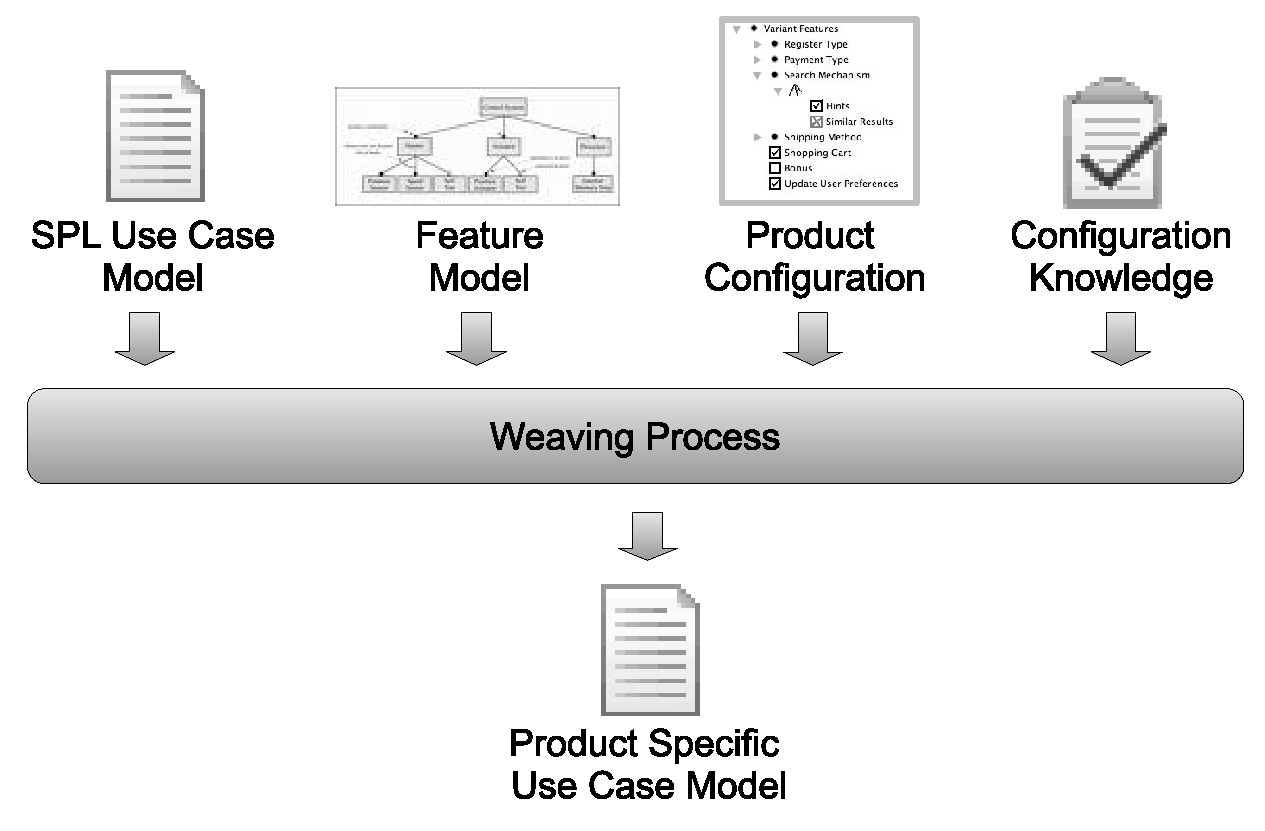
\includegraphics[scale=0.30]{img/weave-process2.eps}
  \caption{Overview of our weaving process.}
  \label{fig:weave-process}
  \end{center}
\end{figure}

\subsection{Feature model}

Feature models have an important contribution to our
weaving process, since they are used for checking if a product
configuration is a valid member of the product line. It is important to note
that we are not proposing a new notation for feature modeling. Here we
only present the features required (Figure~\ref{fig:eshop-fm}) for
understanding the SVCM example.

Based on the feature model of Figure~\ref{fig:eshop-fm}, the \emph{Shopping
Cart}, \emph{Bonus} and \emph{Update User Preferences} features are optional; on
the other hand, the \emph{Shipping Method} feature is mandatory and all products
have to be configured with at least one of its child. Additionally, the
restriction $Shopping\ Cart\ \Leftrightarrow\ Bonus$ states that all
products configured with the shopping cart feature must also be configured with
the bonus feature. More details about feature modeling can be found
elsewhere~\cite{Gheyi:2006aa,Czarnecki:2000aa}.


\subsection{SPL use case model}

This artifact defines scenarios that describe the expected behavior of the SPL's
members. Scenarios might be optional, have parameters, and change (advice) the
behavior of other scenarios. A use case model is composed by \emph{use cases} and
\emph{aspectual use cases}. A use case has a name, a description and a list of
scenarios, which consist of a sequence of steps (pairs of \emph{User action x
System response}). An aspectual use case has a name and a list of advices, which
can be used to extend the behavior of existing scenarios. Differently from
PLUSS and PLUC, our proposed scenarios are not enriched with alternative steps,
product definition, and information related to configurability.
In this SVCM example, we consider the following scenarios and advices:

{\bf Proceed to Purchase:} this mandatory scenario
(Figure~\ref{fig:proceed-to-checkout}) specifies the common behavior that is
required for confirming a purchase. Instances of the product line must be
configured with this scenario. Notice that a parameter
\emph{ShippingMethod} is referenced in Step P2. This parameter (notation
also supported in PLUSS and PLUC) allows the reuse of the \emph{Proceed to
Purchase} scenario for different configurations of \emph{Shipping Method}.

\begin{figure}[h]
\begin{scriptsize}
  \texttt{
   \begin{tabular}{l}
   	 {\bf Id: SC01} 	\\
     {\bf Description:} Proceed to purchase\\
   \end{tabular}
  \begin{center}
  \begin{tabular}{||p{0.1in}||p{1.4in}||p{1.4in}||}
   \hline
       Id & User Action  & System Response \\ \hline \hline
       P1 & Fill in the requested information and select the proceed option.  & Request the shipping method and address.\\  \hline
       P2 & Select one of the available ship methods (\mbox{<SM>}),
       fill in the destination address and proceed. & Calculate the shipping costs. \\  \hline P3 & Confirm the purchase. & Execute the order and send a request to the Delivery System to dispatch the products.
       \mbox{[RegisterPreference]} \\  \hline
  \end{tabular}
  \end{center}
  }
\end{scriptsize}
\caption{Proceed to purchase scenario.}
\label{fig:proceed-to-checkout}
\end{figure}

{\bf Buy Product:} this advice (Figure~\ref{fig:buy-product-scenario}) enables a
customer to buy specific goods from an on-line shopping store. It is only
available in the product line members that are {\bf not} configured with the
\emph{Shopping Cart} and \emph{Bonus} features. Differently from the PLUSS
approach, which directly relates alternative and optional steps to features, in
our approach this kind of information is represented in a distinct artifact: the
configuration knowledge.

The effect of this advice is to introduce an optional behavior {\bf
before} the join points identified in its \emph{pointcut} clause. In this case,
the Step P1 defined in the \emph{Proceed to Purchase} scenario.

\begin{figure}[h]
\begin{scriptsize}
  \texttt{
   \begin{tabular}{l}
   	 {\bf Id: ADV01} 	\\
     {\bf Description:} Buy a specific product\\
     {\bf Before:}  P1
   \end{tabular}
  \begin{center}
  \begin{tabular}{||p{0.1in}||p{1.4in}||p{1.4in}||}
   \hline
       Id & User Action  & System Response \\ \hline \hline
       B1 & Select the buy product option.  & Present the selected product. The user can change the quantity of items he wants to buy. Calculate and show the amount to be paid. \\  \hline
       B2 & Select the confirm option. &  Request payment information. \\  \hline
    \end{tabular}
  \end{center}
  }
\end{scriptsize}
\caption{Buy product advice.}
\label{fig:buy-product-scenario}
\end{figure}

{\bf Buy Products with Shopping Cart and Bonus:} this advice
(Figure~\ref{fig:buy-product-changing-flow}) allows purchasing products
that have been previously added to a customer shopping cart. It extends the
behavior of the \emph{Proceed to Purchase} scenario by introducing the specific
behavior required by the \emph{Shopping Cart} and
\emph{Bonus} features. Therefore, this advice is required by products that
are configured with both \emph{Shopping Cart} and \emph{Bonus} features.

\begin{figure}[h]
\begin{scriptsize}
  \texttt{
   \begin{tabular}{l}
   	 {\bf Id: ADV02} 	\\
     {\bf Description:} Buy products using a shopping-cart\\
     {\bf Before:} P1
   \end{tabular}
  \begin{center}
   \begin{tabular}{||p{0.1in}||p{1.4in}||p{1.4in}||}
   \hline
       Id & User Action & System Response \\ \hline \hline
       C1 & Select the checkout option.  & Present the items in the shopping cart and the amount to be paid. The user can remove items from the shopping cart. \\  \hline
       C2 & Select the confirm option. & Request bonus and payment information. \\  \hline
  \end{tabular}
  \end{center}
  }
\end{scriptsize}
\caption{Buy products with shopping cart advice.}
\label{fig:buy-product-changing-flow}
\end{figure}

As shown in Section~\ref{sec:problem}, PLUSS and PLUC represent all valid
configurations of a scenario in a single artifact. Using our approach, we were
able to separate the common behavior required to confirm a purchase (the base
scenario \emph{Proceed to Purchase}) from its variants, specified in the
\emph{Buy Product} and \emph{Buy Product with Shopping Cart} advices. This allows
our specifications to evolve according to the \emph{Open-Closed}
principle~\cite{Meyer:2000aa}. In our approach, introducing new product variants
require more extensions than changes to the base scenarios.

{\bf Search for
Products:} this mandatory scenario (Figure~\ref{fig:search-products-flow}) allows
the user to search for products. In order to save space, we only present Step S3,
which performs a search based on the input criteria. This step is annotated with
the mark \mbox{{\bf [RegisterPreference]}}, exposing it as a possible extension
point for the behavior of \emph{Register User Preferences}
(Figure~\ref{fig:register-preferences-flow}). The same annotation was assigned to
the Step P3 of \emph{Proceed to Purchase} (Figure~\ref{fig:proceed-to-checkout}).
Such annotations can be referenced by advices, and were proposed as an attempt to
reduce the problem of fragile pointcuts.

%\textcolor{red}{We believe that,
%similarly to the use of annotations, introducing semantic based mechanisms to
%compose scenarios~\cite{Chitchyan:2007aa} does not require significant changes to
%the SVCM weaving process.}
%

\begin{figure}[ht]
\begin{scriptsize}
  \texttt{
   \begin{tabular}{l}
   	 {\bf Id: SC02} 						\\
     {\bf Description:} Search for products. \\
   \end{tabular}
  \begin{center}
   \begin{tabular}{||p{0.1in}||p{1.4in}||p{1.4in}||}
   \hline
       Id & User Action &  System Response \\ \hline \hline
       \ldots & \ldots  & \ldots \\  \hline
       S3 & Inform the search criteria. &  Retrieve the products that satisfy the search criteria. Show a list with the resulting products. [RegisterPreference] \\  \hline
  \end{tabular}
  \end{center}
  }
\end{scriptsize}
\caption{Search for products scenario.}
\label{fig:search-products-flow}
\end{figure}

{\bf Register User Preferences:} this advice updates the user preferences based
on the user's history of searches and purchases. Its behavior can be started {\bf
after} any step assigned to the {\bf [RegisterPreference]} (see the
\emph{pointcut} clause) annotation and is available in products that are
configured with the \emph{Update User Preferences} feature.

\begin{figure}[h]
\begin{scriptsize}
  \texttt{
   \begin{tabular}{l}
   	 {\bf Id: ADV03} 	\\
     {\bf Description:} Register user preferences.\\
     {\bf After}: [RegisterPreference] \\
   \end{tabular}
  \begin{center}
   \begin{tabular}{||p{0.1in}||p{1.4in}||p{1.4in}||}
   \hline
       Id & User Action &  System Response \\ \hline \hline
       R1 & - &  Update the preferences based on the search results or purchased items. \\  \hline
  \end{tabular}
  \end{center}
  }
\end{scriptsize}
\caption{Register user preferences.}
\label{fig:register-preferences-flow}
\end{figure}

In this example, we described several scenarios as being optional or
mandatory. It is important to observe that, in our approach, this kind of
information is not specified in scenario documents. Actually, it is necessary to
consider the relationships between scenarios and features in order to realize
which configurations require a specific scenario.

%As we explained at the
%beginning of this section, each artifact (feature model, product configuration,
%configuration knowledge, and use case model) provides a specific contribution to
%the definition of a SPL's member.


\subsection{Product configuration}\label{subsub:pc}

This artifact identifies a specific SPL member, which is characterized by a valid
configuration of features. Each product configuration should conform to a feature
model (the selected features should obey the feature model relationships and
constraints). For the \emph{eShop} example, two possible configurations are
presented in Figure~\ref{fig:product-config-01-02}. We represent these configurations as a
tree, highlighting which features were selected.


 \begin{figure}[h]
 \begin{center}
  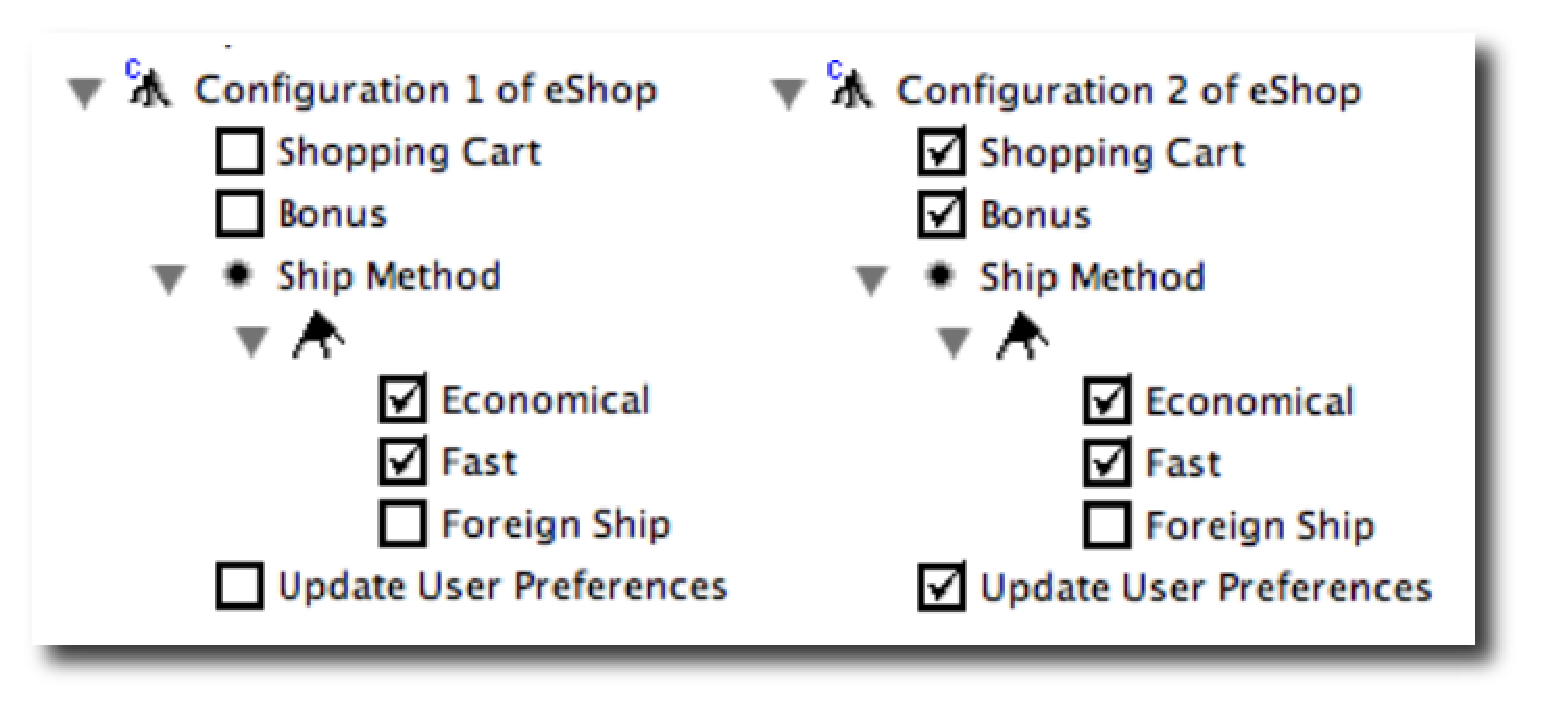
\includegraphics[scale=0.33]{img/pc-04.eps}
   \caption{Examples of product configurations.}
  \label{fig:product-config-01-02}
  \end{center}
\end{figure}

% \begin{figure}[htb] \centerline{
% \mbox{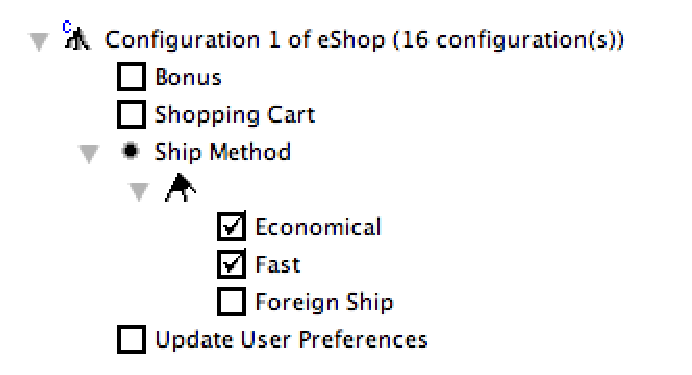
\includegraphics[scale=0.4]{img/pc-01.eps}}
% \mbox{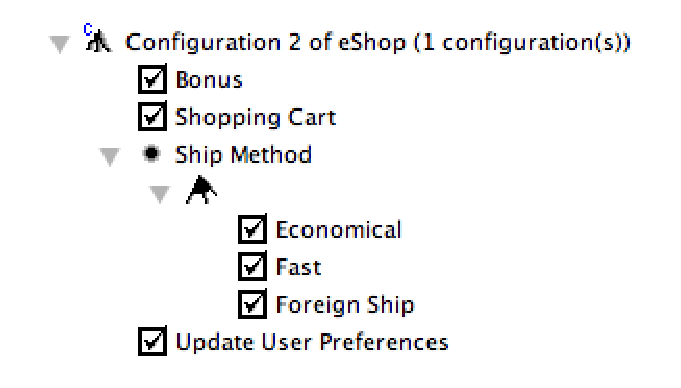
\includegraphics[scale=0.4]{img/pc-02.eps}} } \nocaptionrule
% \caption{Examples of product configurations.} \label{fig:product-config-01-02}
% \end{figure}

The first configuration (on the left side of the
Figure~\ref{fig:product-config-01-02}) defines a product that has no support for
\emph{Shopping Cart}, \emph{Bonus} and \emph{Update User Preferences}.
Additionally, it supports only the economical and fast shipping methods. The
second configuration is more complete, being configured with the features
\emph{Shopping Cart}, \emph{Bonus}, and \emph{Update User Preferences}.

In PLUC, product configurations are scattered through existing scenarios, and
are not explicitly related to features. As discussed in
Section~\ref{sec:problem}, even simple changes in the configuration model might
require a deep review of existing scenarios.

The set of features selected to a specific product (represented as a product
configuration) identifies which tasks must be performed to
generate the corresponding SPL member. In order to do that, the configuration
knowledge (exemplified in what follows) relates feature expressions to such
tasks.

\subsection{Configuration knowledge}

This artifact is represented as a list of configuration items, which relates
feature expressions (written in propositional logic) to the tasks used for
generating specific product. We provide the abstract syntax of this artifact in the appendix. Therefore, the configuration knowledge allows,
during product engineering, the automatic configuration of SPL assets.
Table~\ref{tab:eshop-ck} presents the configuration
knowledge for the running example, enforcing that


\begin{itemize}
\item Both \emph{Proceed to Purchase} (SC01) and \emph{Search for Products}
(SC02) scenarios are mandatory, since their selection is related to the
(mandatory) root feature of the \emph{eShop} product line;

\item The \emph{Buy Product} advice (ADV01) is used in the composition of
products that do not have been configured with both \emph{Shopping Cart} and \emph{Bonus}
features--- if both features were selected for a product, it would be configured
with the \emph{Buy Product with Cart} advice (ADV02). Remember that there is a
mutual dependency between \emph{Shopping Cart} and \emph{Bonus} features. As a
consequence, no product can be configured with just one of them;

\item The \emph{Register User Preferences} advice (ADV03) is not used in a
product composition unless the \emph{Update User Preferences} feature has been
selected; and

\item References to the ``SM'' parameter are bound to the
selected alternatives of the \emph{Shipping Method} feature.

\end{itemize}


\begin{table}[htb]
\begin{small}
\begin{tabular}{||lp{1.4in}||}
\hline
Feature Expression  						& Tasks					 \\ \hline

\multirow{2}{*}{eShop}						& select scenario {\bf SC01} \\
											& select scenario {\bf SC02} \\	\hline
{\bf not} (Shopping Cart {\bf and} Bonus) 	& evaluate advice {\bf ADV01} \\
\hline (Shopping Cart {\bf and} Bonus) 		& evaluate advice {\bf ADV02} 	\\
\hline Update User Preferences 				& evaluate advice {\bf ADV03} \\ \hline
Shipping Method								& bind parameter {\bf SM}\\ \hline
								
\end{tabular}
\end{small}
\caption{Example of configuration knowledge}
\label{tab:eshop-ck}
\end{table}

Three different tasks are used in the configuration knowledge shown in
Figure~\ref{tab:eshop-ck}: \emph{select scenario},
\emph{evaluate advice}, and \emph{bind parameter}. Using the terminology
proposed by Bachmann et al.~\cite{Bachmann:2001aa}, the first task deals with
the source of variability named as \emph{variation in function}; the second one
deals with \emph{variation in control flow}; and the last one deals with
\emph{variation in data}.
Figure~\ref{fig:resulting-purchase} depicts the resulting scenario related to
the purchasing behavior, after evaluating the configuration knowledge of
Table~\ref{tab:eshop-ck}, and considering the second product of
figure~\ref{fig:product-config-01-02}.


\begin{figure}[h]
\begin{scriptsize}
   \texttt{
   \begin{center}
    \begin{tabular}{||p{1.45in}||p{1.45in}||} \hline
       User Action  & System Response \\ \hline \hline
       Select the checkout option.  & Present the items in the shopping
       cart and the amount to be paid. The user can remove items from the
       shopping cart. \\ \hline
       Select the confirm option. & Request bonus and payment information. \\ \hline
       Fill in the requested information and
       select the proceed option.  & Request the shipping method and address.\\ \hline
       Select one of the available ship methods {\bf (Economical, Fast)}, fill
       in the destination address and proceed. & Calculate the shipping
       costs.\\ \hline
       Confirm the purchase. & Execute the order and send a
       request to the Delivery System to dispatch the products. \\ \hline
 	   - &  Update the preferences based on the search results or purchased
 	   items. \\ \hline
    \end{tabular}
   \end{center}
   }
\end{scriptsize}
\caption{Resulting Proceed to Purchase scenario}
\label{fig:resulting-purchase}
\end{figure}		

%There is no artifact similar to our configuration knowledge in
%PLUSS and PLUC approaches. As a consequence, introducing new variants of existing
%features in these techniques usually propagates changes throughout many
%scenarios.


%=================================================================
% Semantica do configuration knowledge
%=================================================================
% \begin{figure*}[hbt]
%  \begin{code}
%   (|->) :: a -> b -> (a,b) -- just a 'syntactic sugar' to build pairs
%   l |-> r = (l,r)
%
%   conf1 = Configuration (``eShop'' |-> selectScenarios[``SC01'', ``SC02''])
%   conf2 = Configuration ('Not' (``ShoppingCart'' 'And' ``Bonus'') |-> evaluateAdvice[``ADV01''])
%   conf3 = Configuration (``ShoppingCart'' 'And' ``Bonus'' |-> evaluateAdvice[``ADV02''])
%   conf4 = Configuration (``UpdateUserPreferences'' |-> evaluateAdvice[``ADV03''])
%   conf5 = Configuration (``ShipMethod'' |-> bindParameter(``ShipMethod'', `ShipMethod''))
%   ...
%
%   ck = [conf1, conf2, conf3, conf4, conf5]
%  \end{code}
% \caption{eShop configuration knowledge}
% \label{fig:ck-running-example}
% \end{figure*}
%
% We can reason about the effect of evaluating a configuration knowledge
% by means of trace models, defined to our context as:
%

%
% \begin{definition}
% A trace model is the set of valid sequences of events
% computed from the product scenarios. Events are labeled as the step ids of a
% scenario. The trace model for a scenario $s$ is given by:.
% \end{definition}
%
% \begin{code}
% traceModel s = traces (steps s)
% where
%   traces [] = [[]]
%   traces (x:xs) = [] : (stepId x) ^ (traces (xs))
%
% (^) :: (a -> [[a]]) -> [[a]]
% x ^ y = [ x:e | e <- y ]
% \end{code}
%
% For instance, Table~\ref{tab:ck-evaluation} presents the resulting trace models,
% after evaluating each configuration item of Figure~\ref{fig:ck-running-example}
% and considering the second product represented in
% Figure~\ref{fig:product-config-01-02}. Notice that the trace model of an empty
% product is the set with just one element: the empty sequence of events (not
% represented in Table~\ref{tab:ck-evaluation}).
%
% \begin{table}[hbt]
%   \begin{tabular}{{||m{0.3in} m{0.1in} p{0.05in} l||}}
%   	\hline
%  	Config 		  & Eval		 & & Trace Model  \\  \hline 	
%  	
%  	$conf1$		  & True	     & & \parbox[t]{2.4in} {
%  									 \raggedright
%  									 <>, <P1>, <P1,P2.sm>, <P1,P2.sm,P3>,
%  									 <S1>, <S1,S2>, <S1,S2,S3> \\
%  								    } 									
%     								\\ \hline
%     $conf2$		  & False	   & & \parbox[t]{2.4in} {
%  								   \raggedright
%  									 <>, <P1>, <P1,P2.sm>, <P1,P2.sm,P3>,
%  									 <S1>, <S1,S2>, <S1,S2,S3> \\
%  								  }
%  								 \\ \hline 										
% 	$conf3$		  & True	   & & \parbox[t]{2.4in} {
%  								   \raggedright
%  									 <>, <C1>, <C1,C2>, <C1,C2,P1>,
% 							         <C1,C2,P1,P2.sm>, <C1,C2,P1,P2.sm,P3>,
%  								     <S1>, <S1,S2>, <S1,S2,S3> \\
%  								   } 								
%  								 \\ \hline
% 	$conf4$		  & True	   & & \parbox[t]{2.4in} {
%  								   \raggedright
% 	                                <>, <C1>, <C1,C2>, <C1,C2,P1>,
% 							        <C1,C2,P1,P2.sm>, <C1,C2,P1,P2.sm,P3>,
% 							        <C1,C2,P1,P2.sm,P3,R1>,
%  								    <S1>, <S1,S2>, <S1,S2,S3>,
%  								    <S1,S2,S3,R1> \\
%  								   }   	
%  								 \\ \hline
% 	$conf5$		  & True	   & & \parbox[t]{2.4in} {
%  								   \raggedright
% 									<>, <C1>, <C1,C2>, <C1,C2,P1>,
% 							     <C1,C2,P1,P2.(Economical,Fast)>,
% 							     <C1,C2,P1,P2.(Economical,Fast),P3>,
% 							     <C1,C2,P1,P2.(Economical,Fast),P3,R1>
%  								 <S1>, <S1,S2>, <S1,S2,S3>,
%  								 <S1,S2,S3,R1> \\   	 							
%  								 }
%  								 \\ \hline	 						  	
%  				
%    \end{tabular}
% \caption{The effect of evaluating configuration items}
% \label{tab:ck-evaluation}
% \end{table}

%=================================================================
%=================================================================




% In what follows, we describe a high level view of the weaving process that
% combines the input languages in order to manage scenario variability.  Then, in
% Section~\ref{sub:modeling-framework} we formally present its semantics in terms
% of our modeling framework.

% \subsubsection{Weaving process}
%
% The weaving process represented in Figure~\ref{fig:weave-process} is responsible for performing the following activities:
%
% {\bf Validation activity:} This activity is responsible for checking if a product configuration is a valid instance of the feature model. If the product configuration is
% valid (it conforms to the relationship cardinalities and constraints of the feature model), the process might proceed.
%
% {\bf Product derivation activity:} This activity takes as input a (valid) product configuration and a configuration knowledge.
% Each feature expression of the configuration knowledge is checked against the product configuration. If the expression
% is satisfied, the related scenarios are assembled as the result of this activity. For the running example,
% Table~\ref{tab:assembled-scenarios} shows the assembled scenarios for the configurations depicted in Figure~\ref{fig:product-config-01-02}.
%
% \begin{table}[h]
% \begin{center}
% \caption{Assembled scenarios} \label{tab:assembled-scenarios}
% \begin{tabular}{ll}
%    \hline\noalign{\smallskip}
%   {\bf Configuration} & {\bf Assembled scenarios} \\
%    \noalign{\smallskip}
%    \hline
%    \noalign{\smallskip}
%     Configuration 1\hspace{15pt} & Proceed to Purchase \\
%                                                    & Search for Products \\
%                                                    & Buy a Product \\
%                              			  & \ldots \\
%    Configuration 2                        & Proceed to Purchase \\
%                              			  & Search for Products	 \\
% 			                           & Buy Products with Cart \\
%                                                    & Register User Preferences \\
%                              & \ldots       \\
%   \hline
% \end{tabular}
% \end{center}
% \end{table}
%
%  {\bf Scenario composition activity:} This activity is responsible for composing the scenarios assembled for a specific product configuration.
% Therefore, the resulting scenarios of the previous activity, which crosscut each other based on the \emph{From step} and \emph{To step clauses}, are woven. The
%  result is a use case model with complete paths (all \emph{From step} and \emph{To step} clauses are resolved).
%
% %  or a trace model (a set of all valid sequences of events extracted from the complete paths).
%
% The complete path is a high level representation, which uses the same constructions of the use case model (scenarios), and is illustrated here as a graph, where each node is labeled with a step id. For example, Figure~\ref{fig:complete-paths} depicts the complete paths for the first and second configurations of our running example. In the left side of the figure,  the composition of \emph{Buy a Product} with \emph{Proceed to Purchase} (branch labeled as B1, B2, P1, P2, P3) and \emph{Search for Product} (branch labeled as S1, S2, S3) scenarios are presented. Contrasting, on the right side of the figure, the results of this activity is presented for the second configuration. In this case, steps B1 and B2 have been replaced by steps V1 and V2 (because \emph{Shopping Cart} and \emph{Bonus} features are selected) and the step  R1 is introduced after steps P3 and S3 (because \emph{Update User Preferences} is selected in this configuration).
%
% %=====================
% % Trace model discussion
% %=====================
%
% %Instead, the trace model can be seen as a low level representation of the use case model. Such notation has a well defined semantic and might
% %be used for model checking and test case generation. Such applications of the trace model are beyond the scope of this paper. More information
% %can be found elsewhere\cite{csp-hoare,csp-roscoe,cfeitosa-sbmf-2006}. Here, the trace model is useful for implementing the last activity of our weave process, binding parameters, and
% %represents all possible sequences of events in a specific product configuration.
%
% %For instance, the trace model for the first configuration is the set of sequences:
%
% %\begin{small}
% %\begin{tabular}{rlc}
% %$Trace_{C1}$ = & \{<>, <idle>, <idle, 1S>, <idle, 1S, 2S>, \\
% %                    & <idle, 1S, 2S, 3S>,  <idle, 1S, 2S, 3S, end>, \\
% %                    & <idle, 1M>, <idle, 1M, 2M>, \ldots, \\
% %                    & <idle, 1M, 2M, 3M, 4M.ShipMethod, 5M, end> \}
% %\end{tabular}
% %\end{small}
%
% %========================
%
% % \begin{figure}[bth]
% % \begin{center}
% % \begin{tiny}
% % \begin{xy}
% % \xymatrix@R=10pt{
% % & *++[o][F-]{idle} \ar[r]\ar[d] & *++[o][F-]{B1} \ar[d]	& *++[o][F-]{idle} \ar[r]\ar[d] & *++[o][F-]{V1} \ar[d] 		\\
% % & *++[o][F-]{S1} \ar[d]  & *++[o][F-]{B2} \ar[d]           & *++[o][F-]{S1} \ar[d]  & *++[o][F-]{V2} \ar[d] 			\\
% % & *++[o][F-]{S2} \ar[d]  & *++[o][F-]{P1} \ar[d]           & *++[o][F-]{S2} \ar[d]  & *++[o][F-]{P1} \ar[d]			\\
% % & *++[o][F-]{S3} \ar[d]  & *++[o][F-]{P2} \ar[d]           & *++[o][F-]{S3} \ar[d]  & *++[o][F-]{P2} \ar[d] 			\\
% % & *++[o][F-]{end} & *++[o][F-]{P3} \ar[l]                     & *++[o][F-]{R1} \ar[d] & *++[o][F-]{P3} \ar[l]   			\\
% % &                         &                                                    &   *++[o][F-]{end}       &
% % }
% % \end{xy}
% % \end{tiny}
% % \caption{Complete paths represented  as a graph}
% % \label{fig:complete-paths}
% % \end{center}
% % \end{figure}
%
% {\bf Binding parameters activity:}  This activity weaves scenarios and product configurations in order to resolve all scenario parameters.
% For example, step P2 in Figure~\ref{fig:proceed-to-checkout} has a reference
%  to the \emph{ShipMethod} parameter, whose domain values are defined in the product configuration. For instance, in the first configuration depicted in Figure~\ref{fig:product-config-01-02}, the parameter \emph{ShipMethod} might assume the values \emph{Economical} or \emph{Fast}.
% In order to reduce the coupling between scenario specifications and feature model, a mapping is used for relating scenario parameters to features. In fact, this mapping is another input artifact of our modeling framework; but it was not represented in Figure because it was just introduced for avoiding explicit dependences between feature and use case models.
% Next, we introduce the modeling framework used to formally describe the weaving processes just presented.
% %===================
% % Trace model discussion
% %===================
%
% %For each trace that contains a parameterized event (or step), this activity creates a new trace for all of the possible parameter values. Consequently, resolving parameters for the trace $<idle,1M,2M,3M,4M.ShipMethod>$ results in the following sequences:
% %
% %\begin{center}
% %\begin{small}
% %\begin{tabular}{c}
% %<idle,1M,2M,3M,4M.Economical>, \\ <idle,1M,2M,3M,4M.Fast>, \\
% %\end{tabular}
% %\end{small}
% %\end{center}


